\section{Trading Strategy}

%----------------------------------------------------
\subsection{Beta-neutral positions on every $(i,j)\in\mathcal B$}
Since we are interested in the individual effect of an article $i\in\D$ in each of the affected firms $j\in\F^i$, we work with the set
$
\mathcal{B}:=\3{(i,j) \mid i\in \D ~\wedge~j\in \F^i }
$, where $\abs{\mathcal{B}}=3410>\abs{\D}=2613$. 
We then fit a market model to each unique pair $(i,j)\in \mathcal{B}$
%consisting of a firm $j\in\F^i$ affected by article $i$ 
on some window of time $\mathcal{M}^i\subset \tilde{\mathfrak{d}}$ before the effective treatment day: 
\footnote{To rigorously define $\mathcal M^i$, we need to work with the index and inverse index functions. 
\begin{itemize}
  \item \textbf{Index Function}. 
Given a finite ordered set $\mathcal{Z}=\left\{z_1, z_2, \ldots, z_n\right\}$, the index function 
$\mathbb{I}_{\mathcal{Z}}: \mathcal{Z} \rightarrow\{1,2, \ldots,|\mathcal{Z}|\}$
%$\mathbb{I}_{\mathcal{Z}}(z)$
 maps an element $z\in\Z$ to its position in the ordered set $\mathcal{Z}$. Formally:
$
\mathbb{I}_{\mathcal{Z}}(z_{\ell})=\ell 
%\quad \text { if and only if } \quad z=z_{\ell} 
~ \text { for } ~ \ell \in\{1,2, \ldots,|\mathcal{Z}|\}
.
$
%where $z_{\ell}$ denotes the ${\ell}$-th element of the ordered set $\mathcal{Z}$.

\item \textbf{Inverse Index Function}. 
The inverse index function 
$\mathbb{I}_{\mathcal{Z}}^{-1}:\{1,2, \ldots,|\mathcal{Z}|\} \rightarrow \mathcal{Z}$
%$\mathbb{I}_{\mathcal{Z}}^{-1}({\ell})$
 retrieves the element $z \in \mathcal{Z}$ corresponding to a given index ${\ell}$.
Formally:
$
\mathbb{I}_{\mathcal{Z}}^{-1}({\ell})=z_{\ell} ~\text { for } ~{\ell} \in\{1,2, \ldots,|\mathcal{Z}|\}
.$
\end{itemize}
For the market model window, we use $\mathbb{I}_{\tilde{\mathfrak{d}}}$ and $\mathbb{I}^{-1}_{\tilde{\mathfrak{d}}} $ applied to the set of trading days $\tilde{\mathfrak d}$. Namely:
$$
\mathcal{M}^i := 
\3{
d\in \tilde{\mathfrak{d}}
\c 
\mathbb{I}^{-1}_{\tilde{\mathfrak{d}}} 
\1{
\mathbb{I}_{\tilde{\mathfrak{d}}} (\tilde{d}_0^i) - {w}_b - {w}_m 
}
\leq d \leq 
\mathbb{I}^{-1}_{\tilde{\mathfrak{d}}} 
\1{ 
\mathbb{I}_{\tilde{\mathfrak{d}}} (\tilde{d}_0^i) - {w}_b 
}
}
,
$$
with a buffer of ${w}_b=10$ trading days before the effective treatment date, and a market model window length of ${w}_m=100$ trading days.



}
%----------------------------------------------------
$$
r_{d}^{j} = \alpha^{(i,j)} + \beta^{(i,j)} r_{d}^M + \epsilon_{ d}^{(i,j)} 
\qquad  
%\t{for}
%~
%\qquad
\forall d \in \mathcal{M}^i
,
$$
%\begin{align*}
%r_{\tilde d}^{j} = \alpha^{(i,j)} + \beta^{(i,j)} r_{\tilde d}^M + \epsilon_{\tilde d}^{(i,j)} 
%\qquad  
%\t{for}
%~
%%\qquad
%\tilde d \in 
%\5{
%\tilde d_0^i - \widetilde{w}_b - \widetilde{w}_m
%~,~
%\tilde d_0^i - \widetilde{w}_b
%}
%,
%\end{align*}
where 
$r_{d}^{j}$ denotes the return of firm $j$ at trading day $d$ in excess of the risk-free asset, which we take to be the daily euro short-term rate (\texttt{\euro STR}),
and 
$r_{d}^M$ denotes the excess return of the market (IBEX-35).  
%----------------------------------------------------
These returns are obtained from the adjusted close price, which corrects the price evolution for corporate actions such as dividends, stock splits, and new stock issuance.\footnote{
The adjusted close price ensures that the returns reflect the true economic gains or losses for an investor holding the stock. 
%
Formally, the return of firm $j$ between two trading days $d_1, d_2\in \tilde{\mathfrak{d}}$ is computed as:
$
r_{d_1:d_2}^{j} = 
%\frac{
(
p_{d_2}^{j,\text{adj}} - p_{d_1}^{j,\text{adj}}
%}{
)/(
p_{d_1}^{j,\text{adj}}
)
%},
$
where $p_{d}^{j,\text{adj}}$ is the adjusted close price of firm $j$ at trading day $d$.
}
%----------------------------------------------------

\mx 
%----------------------------------------------------
The notation overload in the regression coefficients $(\alpha^{(i,j)},\beta^{(i,j)})$ emphasizes the fact that $\alpha$ and $\beta$ are specific to each pair $(i,j)\in\mathcal B$ since the market model is computed for each firm $j\in\F_{\t{IBEX-35}}$ on some specific window of time $\mathcal{M}^i$, which is particular to each article $i\in\D$.
%----------------------------------------------------

\mx 
The reason why we fit a market model to each $(i,j)\in\mathcal B$ is to then apply a market-neutral strategy as in \cite{chan2003stock} and \cite{jiang2021pervasive}. This is an investment approach designed to minimize or eliminate exposure to overall market movements, isolating the performance of a specific firm. 
%The primary goal is to achieve positive returns regardless of the market's direction (up or down). 
In particular, we employ a beta-neutral strategy by buying one unit of firm $j$'s stock and shorting $\beta^{(i,j)}$ units of the market index (i.e.: an ETF replicating the IBEX-35). 

%where $\beta^{(i,j)}$ is the sensitivity of the firm's stock to the market. 

% This approach allows us to isolate the impact of news articles on individual stock performance without the confounding influence of market-wide movements.

%This approach neutralizes the impact of broad market movements, allowing us to focus on the abnormal returns generated by specific news events. 
%This beta-neutral strategy isolate the impact of news articles on individual stock performance without the confounding influence of market-wide movements.


%\mx 
%Based on the estimates $( \alpha^{(i,j)},  \beta^{(i,j)})$, we apply a market-neutral strategy, which is an investment approach designed to minimize or eliminate exposure to overall market movements, isolating the performance of firm $j$. The primary goal is to achieve positive returns regardless of the market's direction (up or down). In this strategy, long positions are taken in firms expected to outperform the market, and short positions are taken in firms expected to underperform. 

%The beta-neutral aspect involves adjusting the portfolio so that the weighted average beta is zero, meaning the portfolio's value should not be affected by market movements. This reduces market risk and focuses on the performance of selected securities. By employing a beta-neutral strategy in this thesis, we aim to isolate the impact of news articles on individual stock performance without the confounding influence of market-wide movements.
%----------------------------------------------------
\mx
This hedged position harvests the idiosyncratic returns from the market model and it only makes sense when firm $j$'s returns are expected to outperform or underperform the market.\footnote{
For expected underperformance of firm $j$, reverse the beta neutral positions: 
sell one unit of firm $j$ and buy $\beta^{(i,j)}$ units of the market index. However, note that this will be handled later by a Trading Rule $(TR)$.
%Note that in the case of expected underperformance of firm $j$, the beta neutral positions should be reversed: sell one unit of firm $j$ and buy $\beta^{(i,j)}$ units of the market index. But for now, there is no need to be concerned with this: the ultimate construction of the positions will be managed by the later introduced Trading Rule $(TR)$.
\mx 
}
The position delivers abnormal returns $AR^{(i,j)}_{d}$ at some trading day $d\geq \tilde{d}_0^i$ given by
%
%Based on the estimates $( \alpha^{(i,j)},  \beta^{(i,j)})$, we compute the returns of a position that buys firm $j$'s stock and sells $ \beta^{(i,j)}$ times the market (by entering into a short position in an ETF that replicates the IBEX-35 Index). This hedged position delivers abnormal returns at trading date $\tilde d$ given by
\begin{align*}
r_{d}^j -  \beta^{(i,j)} r_{d}^M = \alpha^{(i,j)} + \epsilon_{d}^{(i,j)} =: AR^{(i,j)}_{d}
.
\end{align*}
%----------------------------------------------------
The position is taken at the effective treatment date $\tilde d_0^i$ and is maintained over a holding window $\mathcal H^i \subset \tilde{\mathfrak{d}}$ consisting of $L\in\mathbb{N}$ trading days after $\tilde d_0^i$, where $L$ is set to 4 trading days.\footnote{  
The holding period of the position is defined as 
$
\mathcal H^i:=
\3{
d \in \tilde{\mathfrak{d}}
\c 
\tilde{d}_0^i
\leq d \leq 
\mathbb{I}^{-1}_{\tilde{\mathfrak{d}}}\1{\mathbb{I}_{\tilde{\mathfrak{d}}}(\tilde d_0^i)+L}}
%\mathbb{D}_{\tilde{\mathfrak{d}}}\1{\mathbb{I}_{\tilde{\mathfrak{d}}}(\tilde d_0^i)+L}}
$}
%----------------------------------------------------
The justification for this choice of $L$ is made in section A.2 of the Appendix. 

%----------------------------------------------------
\mx 

After having held the beta-neutral position over the holding period $\mathcal H^i$, we obtain a time series of abnormal returns $\{AR_{d}^{(i,j)}\}_{d\in\mathcal H^i}$ from where we can obtain the usual performance metrics. First, the average daily log returns are obtained as
$$
\mu^{(i,j)} = \frac{1}{{{L}}+1} 
%\sum_{d=\tilde d_0^i }^{\tilde d_0^i + {{L}}} 
\sum_{d\in \mathcal H^i}
\ln\4{1+AR_d^{(i,j)}}
~,
$$
%$
%\mu_{{{L}}}^{(i,j)}
%=
%\1{1+CAR_{{{L}}}^{(i,j)}}^{1/({{L}}+1)}-1,
%$
Then, the standard deviation is given by
$$
\sigma^{(i,j)}
=
\sqrt{
\frac{1}{{{L}}}
\sum_{d\in \mathcal H^i}
%\sum_{d=\tilde d_0^i }^{\tilde d_0^i + {{L}}} 
[
\ln(1+AR_d^{(i,j)}) - \mu^{(i,j)}
]
^2}
~.
$$

\mx 
And finally, the annualized Sharpe Ratio can be obtained by scaling the daily Sharpe Ratio by the square root of ${252}$, which are the typical number of trading days in a year according to the Spanish calendar. 
%.  $\sqrt{|\tilde{\mathfrak d}_y|}$
%$
%\sigma_{{{L}}}^{(i,j)}
%= \sqrt{\frac{1}{{{L}}} \sum_{d=\tilde d_0^i}^{\tilde d_0^i + {{L}}} 
%\1{ AR_d^{(i,j)} -\mu_{{{L}}}^{(i,j)} }^2}
%$
$$
SR^{(i,j)} =
\sqrt{252}~
\frac{
\mu^{(i,j)}
}{
\sigma^{(i,j)}
}
%\sqrt{|\tilde{\mathfrak d}_y|}
~.
$$
%%%%%%%%%%%%%%%%%%%%%%%%%%%%%%%%%%%%%%%%%%%%%%%%%%%%%
\subsection{Optimal Cluster Selection}
%%%%%%%%%%%%%%%%%%%%%%%%%%%%%%%%%%%%%%%%%%%%%%%%%%%%%

After taking beta-neutral positions on each pair $(i,j)\in\mathcal B$ and holding them over some window $\mathcal H^i$, we can obtain a measure of how profitable the positions are on average for articles that belong to the same cluster $g\in\mathcal G$. For this purpose, let $\mathcal{B}_g$ denote the set of all article and firm pairs such that the article belongs to some cluster $g\in\mathcal G$. 
$$
\mathcal{B}_g:= \{(i,j) \mid (i,j)\in\mathcal{B} ~\wedge~ i \in \D_g \}
.
$$
The average Sharpe Ratio associated to each cluster is
$$
\overline{S R}_g=\frac{1}{\left|\mathcal{B}_g\right|} \sum_{(i,j) \in \mathcal{B}_g} S R^{(i,j)}
,
$$
and it provides a measure of the performance of the beta-neutral positions in each cluster. 


%
%%----------------------------------------------------
%%----------------------------------------------------
%\begin{figure}[H]
%  \centering
%	\begin{subfigure}[b]{0.45\textwidth}
%		 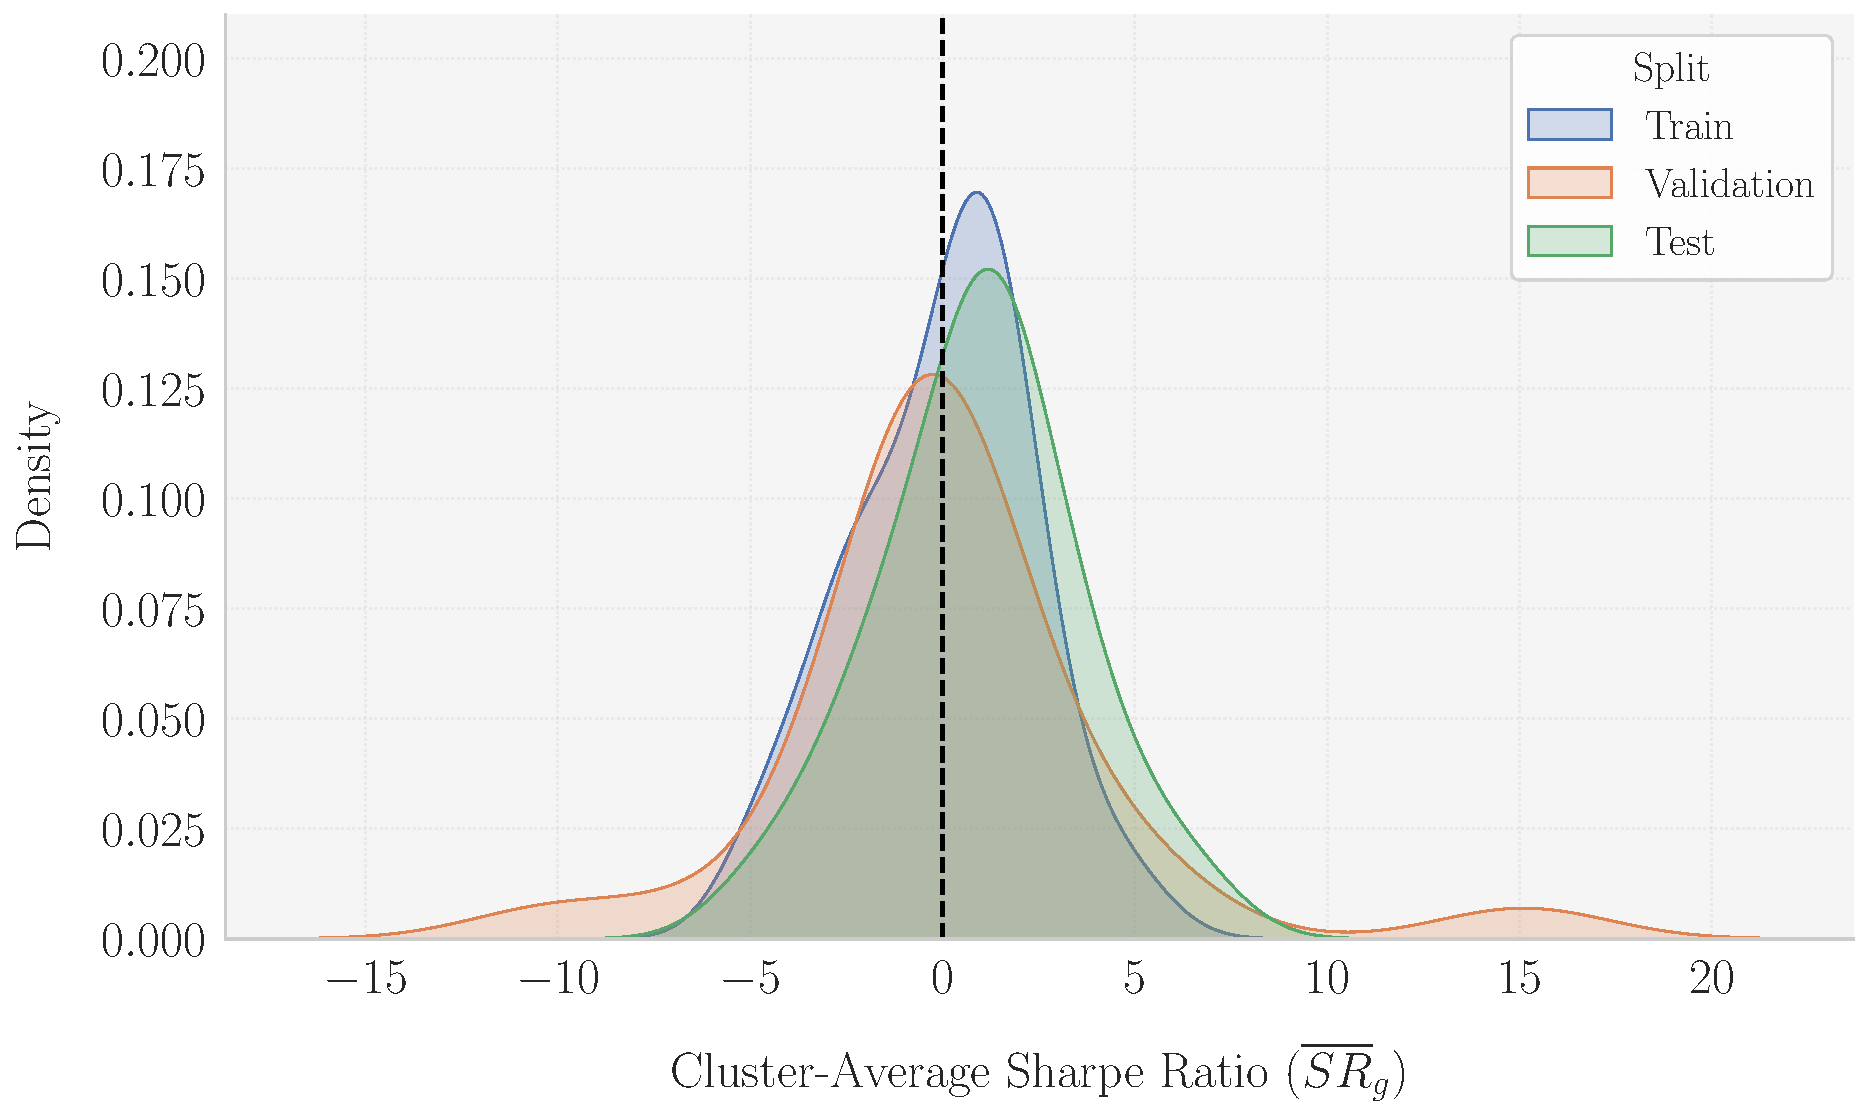
\includegraphics[scale=0.3]{/Users/jesusvillotamiranda/Library/CloudStorage/OneDrive-UniversidaddeLaRioja/CEMFI/__MSc__/__Second_year__/6th_Term/MasterThesis/__Output/KMeans_Cluster-Avg_SR_Distribution.pdf}
%	\end{subfigure}
%	\hfill
%	\begin{subfigure}[b]{0.45\textwidth}
%		  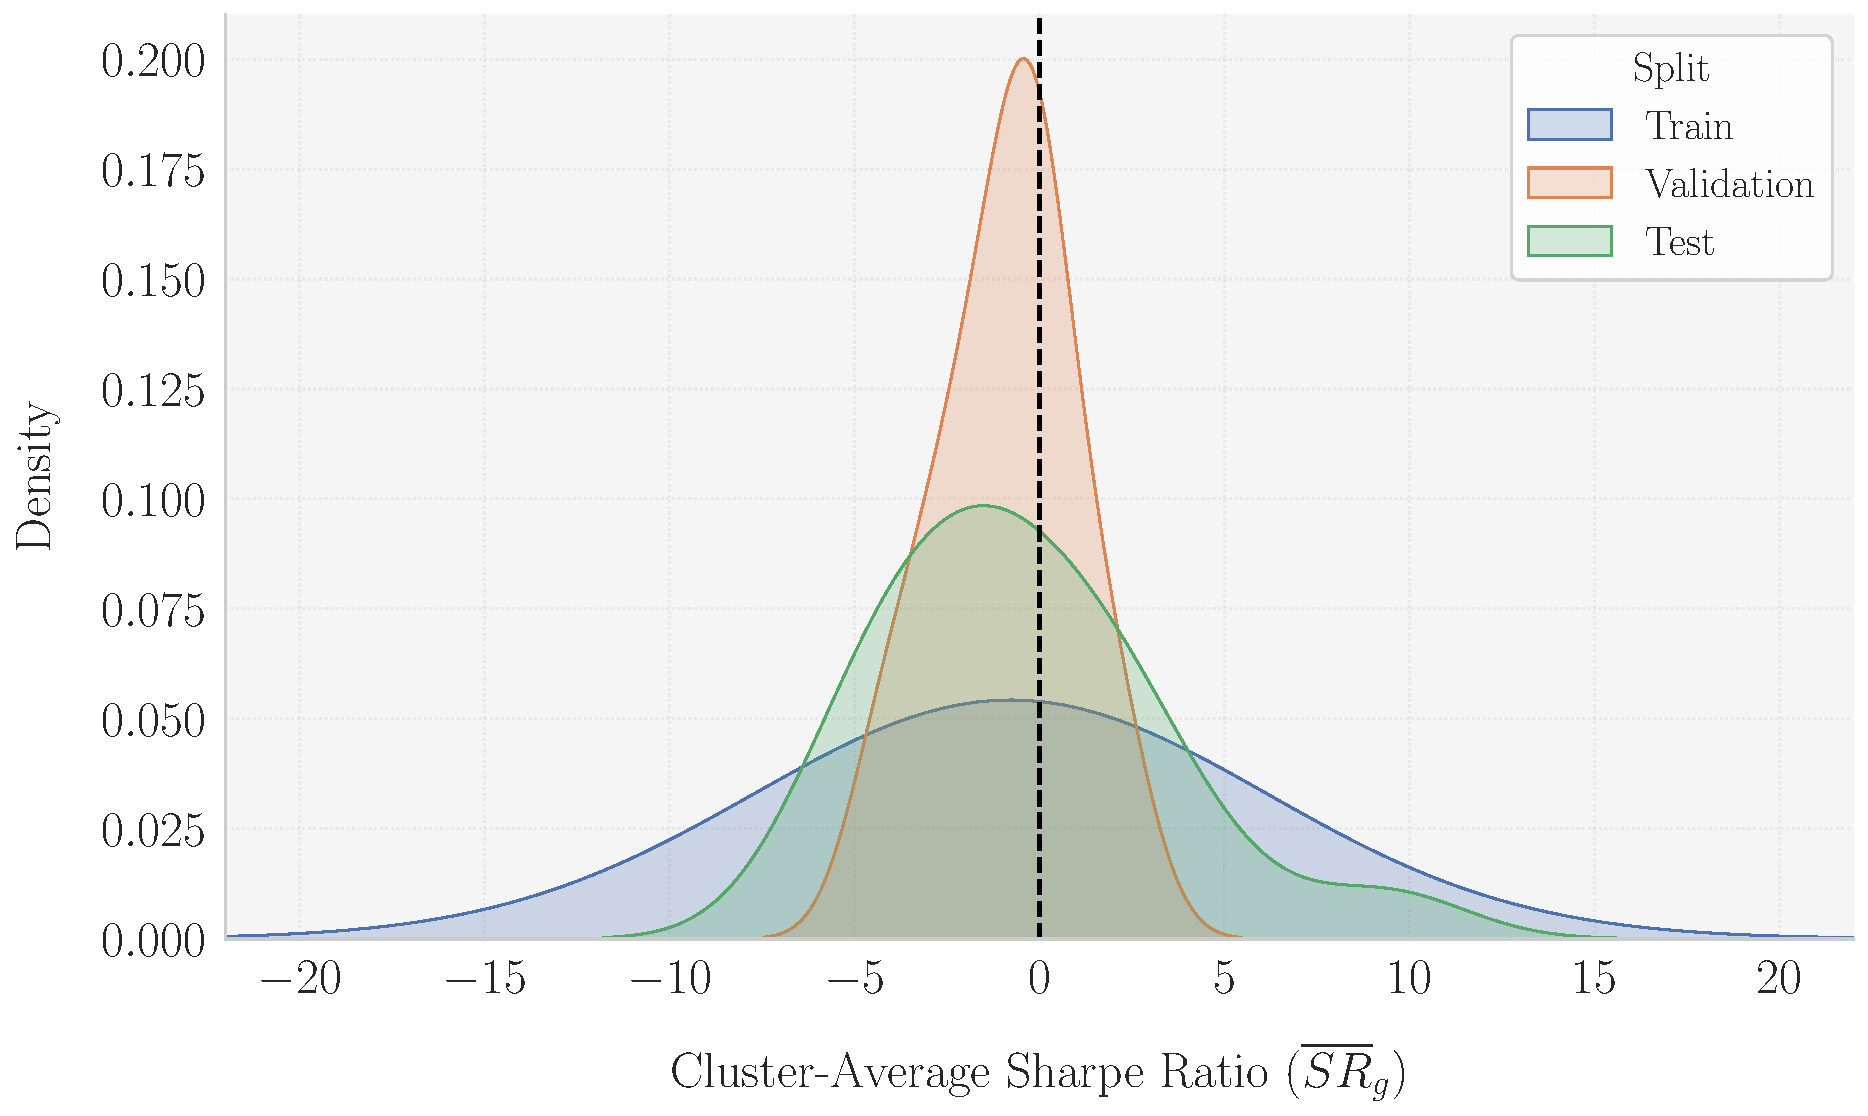
\includegraphics[scale=0.3]{/Users/jesusvillotamiranda/Library/CloudStorage/OneDrive-UniversidaddeLaRioja/CEMFI/__MSc__/__Second_year__/6th_Term/MasterThesis/__Output/LLAMA_Cluster-Avg_SR_Distribution.pdf}
%	\end{subfigure}
%
%
%%  \caption{}
%\end{figure}
%
%%----------------------------------------------------
%%----------------------------------------------------

%%%%%%%%%%%%%%%%%%%%%%%%%%%%%%%%%%%%%%%%%%%%%%%%%%%%%
%%%%%%%%%%%%%%%%%%%%%%%%%%%%%%%%%%%%%%%%%%%%%%%%%%%%%
%%%%%%%%%%%%%%%%%%   KMEANS   %%%%%%%%%%%%%%%%%%%%%%%
%%%%%%%%%%%%%%%%%%%%%%%%%%%%%%%%%%%%%%%%%%%%%%%%%%%%%
%%%%%%%%%%%%%%%%%%%%%%%%%%%%%%%%%%%%%%%%%%%%%%%%%%%%%
In the case of KMeans embeddings, the distribution of cluster-average Sharpe Ratios for across the different clusters is plotted in \cref{fig:KMeans_distr_avg_SR}. In the validation set, they are centered at 0, but we observe some outliers with unusually low and high average $SR$. On the other hand, the distributions in the train and test data are slightly skewed to the right and show no presence of substantial outliers.

%----------------------------------------------------
\inserthere{fig:KMeans_distr_avg_SR}
\begin{figure}[H]
  \centering
  \caption{Distribution of Embeddings-based Cluster-Average Sharpe Ratios $(\overline{SR}_g)$ by Split}
  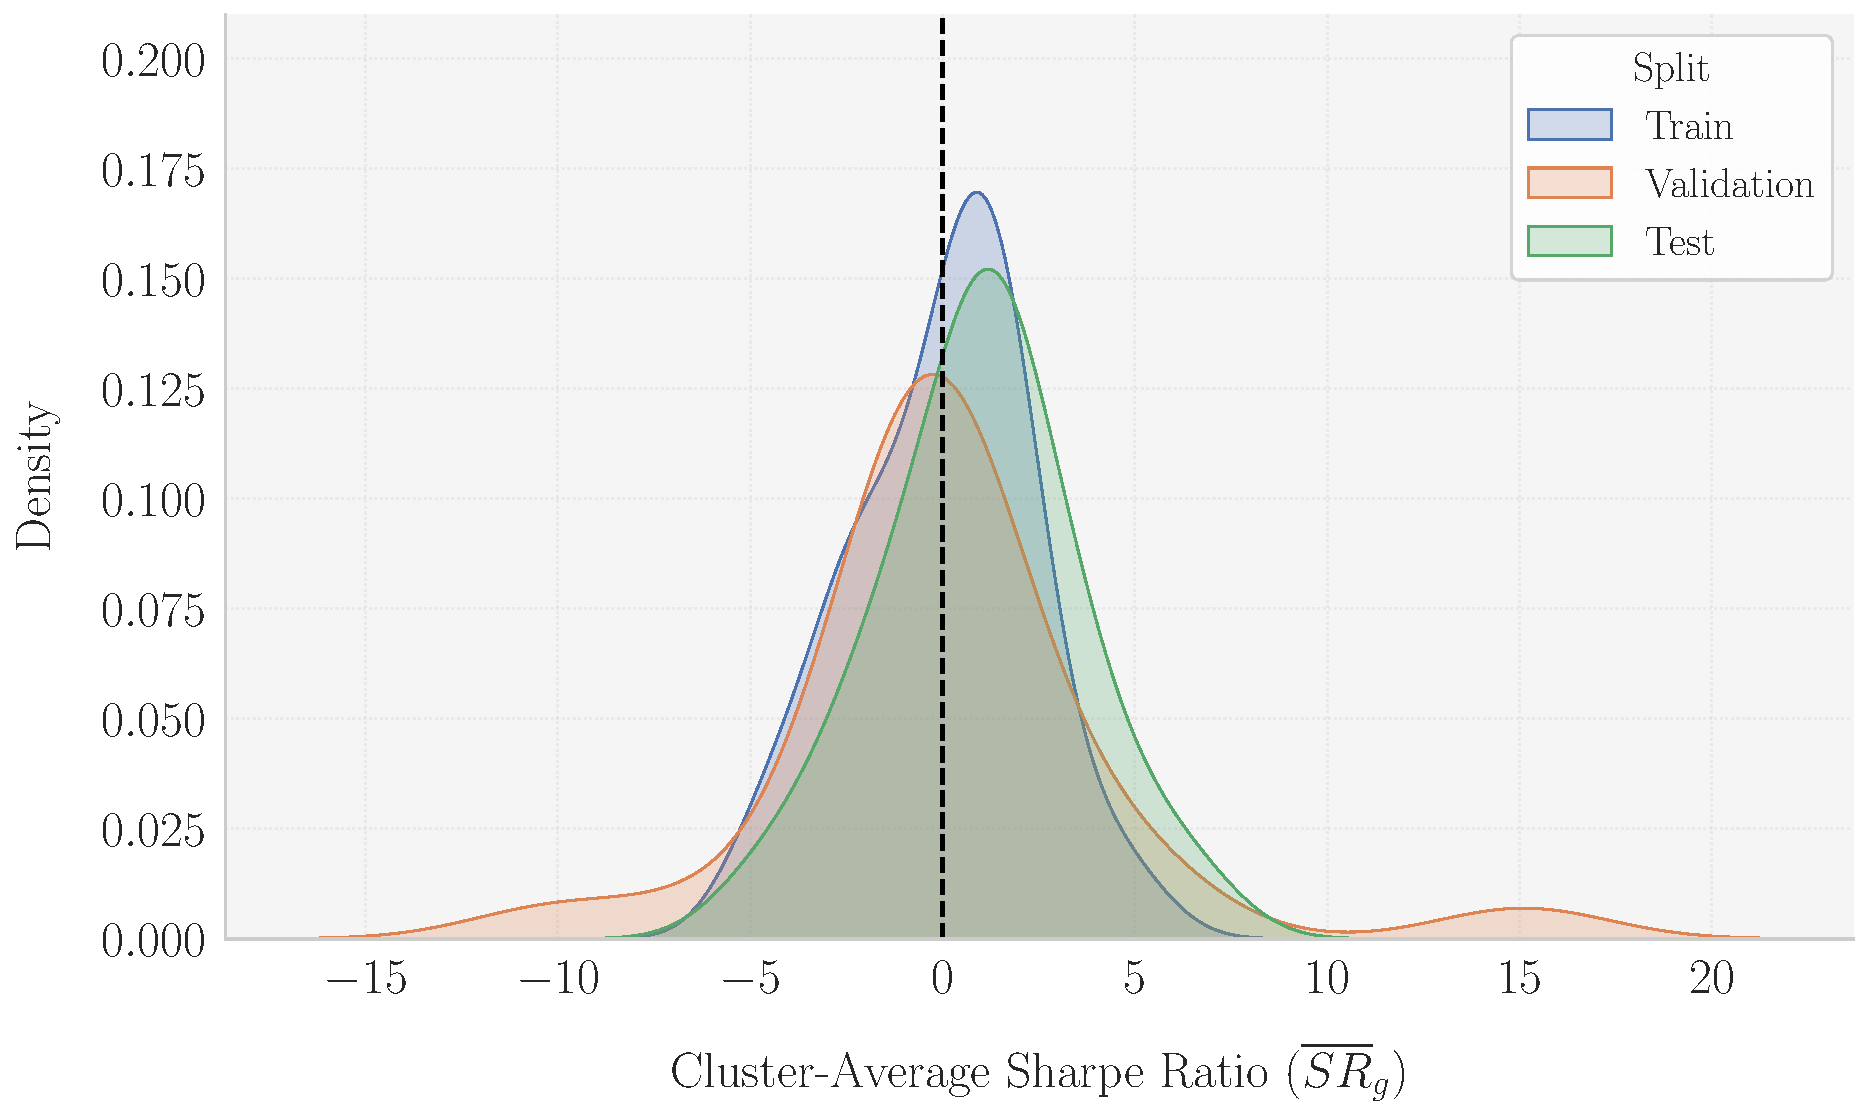
\includegraphics[scale=0.45]{/Users/jesusvillotamiranda/Library/CloudStorage/OneDrive-UniversidaddeLaRioja/CEMFI/__MSc__/__Second_year__/6th_Term/MasterThesis/__Output/KMeans_Cluster-Avg_SR_Distribution.pdf}
\label{fig:KMeans_distr_avg_SR}
\subcaption*{\textit{Note: This figure shows the distribution of cluster-average Sharpe Ratios $(\overline{SR}_g)$ for the embeddings-based KMeans clusters across the different data splits: training, validation, and test sets. Each Sharpe Ratio is computed as the average of beta-neutral positions associated with articles in a given cluster. In the validation set, the distribution is centered around 0, with a few outliers showing unusually high or low Sharpe Ratios. Conversely, the distributions in the training and test sets are slightly skewed to the right, suggesting better performance in certain clusters, with no significant presence of outliers.}}

\end{figure}
%----------------------------------------------------


%%%%%%%%%%%%%%%%%%%%%%%%%%%%%%%%%%%%%%%%%%%%%%%%%%%%%
%%%%%%%%%%%%%%%%%%%%%%%%%%%%%%%%%%%%%%%%%%%%%%%%%%%%%
%%%%%%%%%%%%%%%%%%%%   LLM   %%%%%%%%%%%%%%%%%%%%%%%%
%%%%%%%%%%%%%%%%%%%%%%%%%%%%%%%%%%%%%%%%%%%%%%%%%%%%%
%%%%%%%%%%%%%%%%%%%%%%%%%%%%%%%%%%%%%%%%%%%%%%%%%%%%%
%\bblue{\noindent \Vhrulefill
%
%\noindent \Vhrulefill [~~LLM~~] \Vhrulefill
%
%\noindent \Vhrulefill}

In the case of LLM-based clustering,  
%the same fashion as before, we can plot the distribution of cluster-average Sharpe Ratios for each data split (\cref{fig:LLM_cluster-average-SR-by-split}). Different from before,
 all distributions are left-skewed. The distribution in the training sample has fat tails which severely contrasts with the light-tailed distribution of the validation sample. In the test data, we observe a bell-shaped distribution with some accumulation of mass at high $SR$s (between 5 and 15), indicating stronger performance in some clusters.
%----------------------------------------------------
\inserthere{fig:LLM_cluster-average-SR-by-split}
\begin{figure}[H]
  \centering
  \caption{Distribution of LLM-based Cluster-Average Sharpe Ratios $(\overline{SR}_g)$ by Split}
  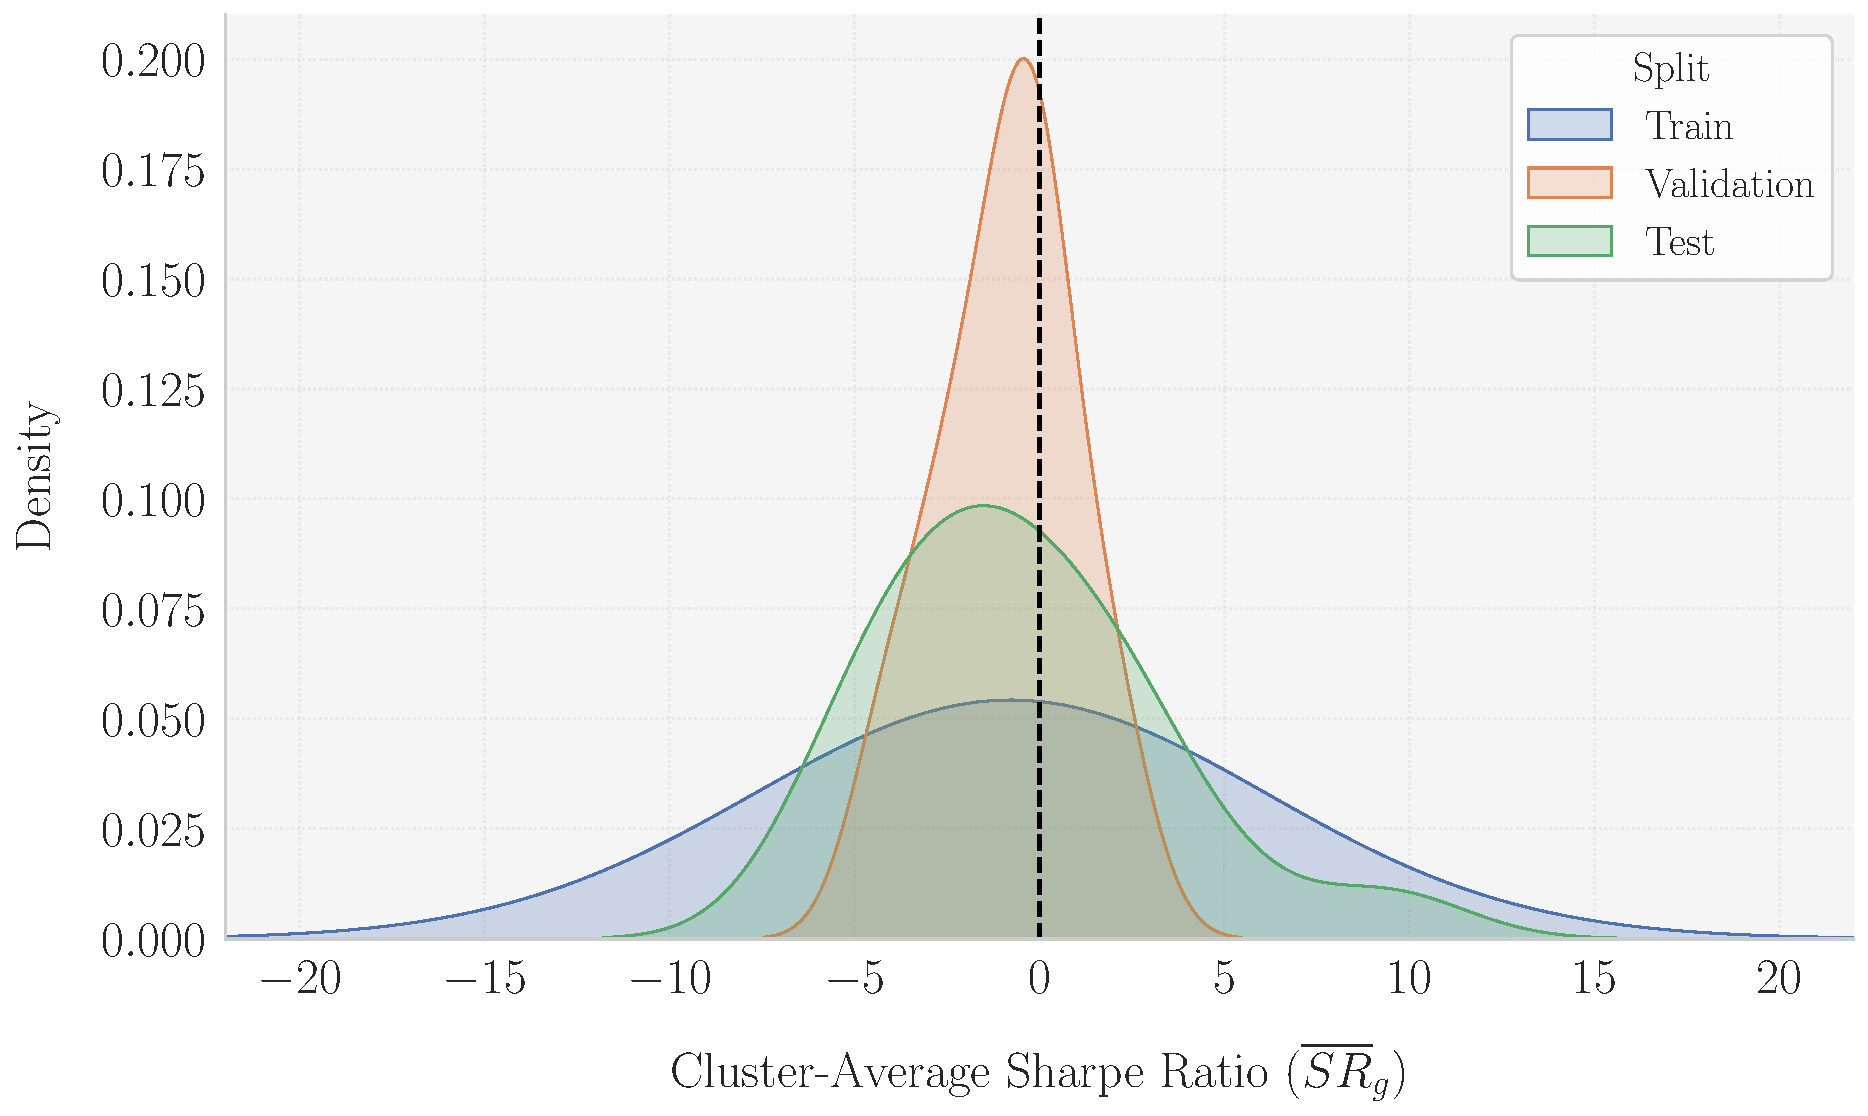
\includegraphics[scale=0.5]{/Users/jesusvillotamiranda/Library/CloudStorage/OneDrive-UniversidaddeLaRioja/CEMFI/__MSc__/__Second_year__/6th_Term/MasterThesis/__Output/LLAMA_Cluster-Avg_SR_Distribution.pdf}
  \label{fig:LLM_cluster-average-SR-by-split}
 \subcaption*{\textit{Note: This figure presents the distribution of cluster-average Sharpe Ratios $(\overline{SR}_g)$ for the LLM-based clustering across the training, validation, and test data splits. All distributions exhibit left-skewness, indicating a higher frequency of lower Sharpe Ratios across clusters. The training data shows a distribution with fat tails, suggesting the presence of extreme values, while the validation data exhibits a much lighter-tailed distribution. In the test data, the distribution is more bell-shaped, with a notable concentration of Sharpe Ratios in the range of 5 to 15, indicating stronger performance in some clusters.}}

\end{figure}
%----------------------------------------------------


%%%%%%%%%%%%%%%%%%%%%%%%%%%%%%%%%%%%%%%%%%%%%%%%%%%%%
%%%%%%%%%%%%%%%%%%%%%%%%%%%%%%%%%%%%%%%%%%%%%%%%%%%%%
%%%%%%%%%%%%%%%%%   ALGORITHMS   %%%%%%%%%%%%%%%%%%%%
%%%%%%%%%%%%%%%%%%%%%%%%%%%%%%%%%%%%%%%%%%%%%%%%%%%%%
%%%%%%%%%%%%%%%%%%%%%%%%%%%%%%%%%%%%%%%%%%%%%%%%%%%%%

\mx
The goal is to now design an algorithm that exploits this information to select the best clusters for the trading strategy. In the remainder of this section, we propose two algorithms. First, an algorithm developed on validation data that will select the clusters maximizing the performance for that split (\qquote{greedy}), and second, an algorithm that will exploit the information from both, training and validation data (higher information set), and whose objective will be to select the most stable clusters among both splits (\qquote{stable}). 


%----------------------------------------------------
%By exploiting the Sharpe Ratios of the beta-neutral positions, we can obtain a simple measure of the profitability of each cluster. In particular, by averaging the annualized Sharpe Ratios of the positions associated to articles that belong to the same cluster. 
%%----------------------------------------------------
%We can then average the annualized Sharpe Ratios of the positions associated to articles that belong to the same cluster. 
%%That is, for each cluster $g$, we compute the average Sharpe Ratio by averaging the Sharpe Ratios of all pairs $(i,j)$ where $i$ belongs to cluster $g$. 
%%--------------- OPTION 1---------------------
%Define $\mathcal{B}_g$ as the set of all pairs $(i,j)\in\mathcal{B}$ such that article $i$ belongs to cluster $g$
%$$
%\mathcal{B}_g:= \{(i,j) \mid (i,j)\in\mathcal{B} ~\wedge~ i \in \D_g \}
%.
%$$
%%--------------- OPTION 2--------------------------- 
%%Formally, let $\mathcal{B}_g$ be the set of all pairs $(i,j)$ such that article $i$ belongs to cluster $g$. 
%%$$\mathcal{B}_g := \{(i,j) \mid  \mbf e^i \in \D_g \}$$
%%----------------------------------------------------
%The average Sharpe Ratio for cluster $g$, denoted as $\overline{S R}_g$, is given by:
%$$
%\overline{S R}_g=\frac{1}{\left|\mathcal{B}_g\right|} \sum_{(i,j) \in \mathcal{B}_g} S R_{{{L}}}^{(i,j)}
%$$


\subsubsubsection{Greedy Algorithm}

The greedy selection of clusters is done in the validation sample 
$
\mathcal{B}_g^{val}:= \{
%(i,j) \mid 
(i,j)\in\mathcal{B} 
%~\wedge~
 \mid 
  i \in \D_g^{val} \}
~,
$
from where we compute the cluster-average $\overline{S R}_g^{val}$ for each $g\in\G$.
%
%\mx 
%----------------------------------------------------
Define $\mathcal G_{SR^+}^{val}:=\{ g\in \mathcal G \mid \overline{SR}_g^{val} >0\}$ and $\mathcal G_{SR^-}^{val}:=\{ g\in \mathcal G \mid \overline{SR}_g^{val} <0\}$ as the sets of clusters with positive and negative Sharpe Ratios in the validation sample. Obviously, we will be interested in taking long positions when reading an article that is clustered in some $g\in \mathcal G_{SR^+}^{val}$, and short positions in clusters $g\in \mathcal G_{SR^+}^{val}$. 


\mx 
%----------------------------------------------------
However, our trading strategy will not trade every cluster $g\in\G$. Instead, it will select the clusters from $\mathcal G_{SR^+}$ and $\mathcal G_{SR^-}$ that lead the to most profitable trades. 
To identify such clusters, we rank them by their average Sharpe Ratio. Define the ranking function $\mathfrak{R}: \mathcal{G} \to \3{1, \ldots, k^*}$ such that
$$
\mathfrak{R}_g^{val}
=
\sum_{h \in \mathcal{G}} 
\mathbf{1}\1{
\overline{S R}_h^{val} \geq \overline{S R}_g^{val} 
}
$$
where $\mathbf{1}(\cdot)$ is the indicator function which equals 1 if the condition inside is true and 0 otherwise.
%$$
%\overline{SR}^{val}_{{{\varkappa}}_1}\geq  \overline{SR}^{val}_{{{\varkappa}}_2} \geq \ldots \geq \overline{SR}^{val}_{{{\varkappa}}_k}
%$$
%where ${{\varkappa}}_1, {{\varkappa}}_2, \ldots, {{\varkappa}}_{k^*}\in\G$ 
%%denote the indices of the sorted clusters 
%are the clusters sorted in descending order
%such that the subindices $\ell=1,...,k^*$ denote the position of cluster $\varkappa_{\ell}$ in the ranking.

\mx
%----------------------------------------------------
The number of traded clusters on either side (long and short) will be upper-bounded by some hyperparameter of our choice $\theta \in \mathbb{N}$
%$\theta \in \{2 m \mid m \in \mathbb{N}\}$ 
which we set proportional to the number of clusters. Namely, $\theta =\integer{\rho k}$ for some $\rho\in(0,1)$, which has been set to $\rho=0.5$ (this choice is justified in section A.2. of the Appendix).
%$\theta\propto k^*$.
%$\theta \in \{2 m \mid m \in \mathbb{N}\}$, which we set proportional to $k^*$.
%$\theta \in\mathbb{E^+}$, where $\mathbb{E}^{+}=\{2 k \mid k \in \mathbb{N}\}$. 
The actual number of traded clusters will not be exactly $\theta$ as there is a natural bound coming from the cardinalities of $\mathcal G_{SR^+}$ and $\mathcal G_{SR^-}$. Hence, the actual number of long and short-traded clusters will be
%$\theta^+$ and $\theta^-$, which are defined as
$
\theta^+ := \min(\theta, ~|\mathcal G_{SR^+}|)
%\quad  
~\t{and}~
%\quad
\theta^- := \min(\theta, ~|\mathcal G_{SR^-}|)
.
$
%
%\mx
%----------------------------------------------------
The set of traded clusters $\mathcal G_{\theta}$ is defined as:
$$
\G_\theta := 
\3{
g \in \mathcal G 
\mid 
1\leq \mathfrak{R}_g^{val} \leq \theta^+
~\vee~ 
k^* -\theta^- < \mathfrak{R}_g^{val} \leq k^*
} 
= 
\G_{\theta}^+ \cup \G_{\theta}^-
~,
$$
where
$
\G_{\theta}^+ := 
\{ g \in\G \mid 
%\varkappa_{\ell} \in \G_{SR^+} \wedge
1\leq \mathfrak{R}_g^{val} \leq \theta^+
\}
$
is the set of long-traded clusters,
%and
$
\G_{\theta}^- := 
\{ g \in\G \mid 
%\varkappa_{\ell} \in \G_{SR^-} \wedge
k^*-\theta^-
< \mathfrak{R}_g^{val} \leq 
k^*
\}
$
is the set of short-traded clusters 
and, clearly, $\abs{\G_{\theta}}=\theta^+ + \theta^- $.\footnote{
Alternatively, we could trade the same number of clusters in the long and short side by defining a unique 
$
\theta^* := \min\1{\theta, |\mathcal G_{SR^+}|, |\mathcal G_{SR^-}| }
%,
$
such that
%In this case, we would have
$
\G_\theta := 
\3{
g \in \mathcal G 
\mid 
1\leq \mathfrak{R}_g^{val} \leq \theta^*
~\vee~ 
k^*-\theta^* < \mathfrak{R}_g^{val} \leq k^*
} 
%= \G_{\theta}^+ \cup \G_{\theta}^-
%.
$
and 
$\abs{\G_\theta}=2\theta^*$.
}
In the appendix, we can find the formal design of this algorithm (\cref{alg:greedy_selection}).

%%%%%%%%%%%%%%%%%%%%%%%%%%%%%%%%%%%%%%%%%%%%%%%%%%%%%
\subsubsubsection{Stable Algorithm}
%%%%%%%%%%%%%%%%%%%%%%%%%%%%%%%%%%%%%%%%%%%%%%%%%%%%%

In this case, we prioritize the stability of the cluster rankings by ensuring that the traded clusters minimize the rank difference of the cluster-average Sharpe Ratios between the training and validation samples. 
To begin, we compute the rank of each cluster based on the average Sharpe Ratios in both the training and validation samples. This delivers $\{\mathfrak{R}_g^{tr}\}_{g\in\G}$ and $\{\mathfrak{R}_g^{val}\}_{g\in\G}$, which provides a measure of the relative performance of the clusters within each sample.
%The ranks for some cluster $g\in\G$ are denoted as $\mathfrak{R}_{g}^{tr}$ for the training sample and $\mathfrak{R}_{g}^{val}$ for the validation sample. These ranks indicate the relative performance of the clusters within each sample. 
%For each cluster $\varkappa$, we calculate:
%\begin{itemize}
%    \item $\mathfrak{R}_{\varkappa}^{tr}$: The rank of the average Sharpe Ratio $\overline{SR}_{\varkappa}^{tr}$ among all clusters in the training sample.
%    \item $\mathfrak{R}_{\varkappa}^{val}$: The rank of the average Sharpe Ratio $\overline{SR}_{\varkappa}^{val}$ among all clusters in the validation sample.
%\end{itemize}

\mx 
Next, we calculate the absolute difference in ranks between the training and validation samples for each cluster, which allows us to measure the stability of each cluster's performance between the two samples
%This rank difference, denoted as $\delta_{g}$, is given by the absolute difference between $\mathfrak{R}_{g}^{tr}$ and $\mathfrak{R}_{g}^{val}$
$$
\delta_{g} := | \mathfrak{R}_{g}^{tr} - \mathfrak{R}_{g}^{val} |
~.
$$

Clusters are then sorted based on their rank differences $\delta_{g}$ in descending order. To do this, we can simply compute the ranking of the ranking differences as
$$
\mathfrak{R}(\delta_g) := \sum_{h\in\G} \mbf{1}\1{\delta_g \geq  \delta_h }
.
$$
Next, we select the top $2\theta\in\mathbb{N}$ clusters with the smallest rank differences, indicating the most stable clusters across the training and validation samples. The selected clusters now are
%denoted as $\mathcal{G}_{\theta}$
$$
\mathcal{G}_{\theta} = 
\3{
g\in\G \c 1 \leq \mathfrak{R}(\delta_g) \leq 2\theta 
}
.
$$

Finally, we determine the sets of long and short-traded clusters based on the average Sharpe Ratios in both the training and validation samples. In particular, the set of long-traded clusters ($\mathcal{G}_{\theta}^{+}$) are the ones that have positive average Sharpe Ratios in both, training and validation samples
$$
\mathcal{G}_{\theta}^{+} = \{g \in \mathcal{G}_{\theta} \mid \overline{SR}_{g}^{tr} > 0 ~\wedge~ \overline{SR}_{g}^{val} > 0\}
,
$$
and by symmetry, short-traded clusters ($\mathcal{G}_{\theta}^{-}$) are the ones that have negative average Sharpe Ratios in both, training and validation samples
$$
\mathcal{G}_{\theta}^{-} = \{g \in \mathcal{G}_{\theta} \mid \overline{SR}_{g}^{tr} < 0 ~\wedge~ \overline{SR}_{g}^{val} < 0\}
~.
$$


This approach ensures that we select the most stable clusters for trading, reducing the risk associated with rank variability between the training and validation samples, and ensuring that the direction of the signal is consistent across the two splits. The final output consists of the sets of long-traded and short-traded clusters, which are then used to implement the trading strategy.


The implementation of the algorithm is methodically presented in the Appendix (\cref{alg:rank_stability}).


%%%%%%%%%%%%%%%%%%%%%%%%%%%%%%%%%%%%%%%%%%%%%%%%%%%%%
%%%%%%%%%%%%%%%%%%%%%%%%%%%%%%%%%%%%%%%%%%%%%%%%%%%%%
%%%%%%%%%%%%%%%%%%   KMEANS   %%%%%%%%%%%%%%%%%%%%%%%
%%%%%%%%%%%%%%%%%%%%%%%%%%%%%%%%%%%%%%%%%%%%%%%%%%%%%
%%%%%%%%%%%%%%%%%%%%%%%%%%%%%%%%%%%%%%%%%%%%%%%%%%%%%

%----------------------------------------------------
\inserthere{tab:KMeans_Clusters_Signal}

\begin{table}[H]
\centering
{\fontsize{11}{12.5}\selectfont
\caption{Mapping of embeddings-based KMeans clusters to Trading Signals}
%\begin{tabular}{|c|L{13cm}|c|c|} 
\begin{tabular}{cL{13cm}cc} 
\hline \Xhline{2\arrayrulewidth}
%\rowcolor{gray!10}
\multicolumn{2}{c}{\textbf{Cluster}} & \textbf{Greedy} & \textbf{Stable} \\ \hline \Xhline{2\arrayrulewidth}
0 & Miscellaneous (Colonial, Acciona, Amadeus, Grifols, Endesa, IAG, Bankinter...) &  \textcolor{darkred}{\textsc{short}} &  \\ \hline
1 & Quarterly \& Semi-Annual Earnings Reports &  \textcolor{darkred}{\textsc{short}} &  \\ \hline
2 & BBVA \& Sabadell: Financial Performance \& Strategic Movements &  \textcolor{darkred}{\textsc{short}} &  \\ \hline
3 & Telef�nica \& Cellnex: Telecommunications Tower Sales \& Market Dynamics &  \textcolor{darkgreen}{\textsc{long}} & \textcolor{darkgreen}{\textsc{long}} \\ \hline
4 & CaixaBank: Mergers and Strategic Moves in the Banking Sector &   &  \\ \hline
5 & Telef�nica, Indra, \& M�sM�vil: Regulatory and Strategic Moves in Telecom &  \textcolor{darkgreen}{\textsc{long}} &  \\ \hline
6 & Siemens Gamesa: Supply Agreements, Profitability Targets in Renewable Energy &  \textcolor{darkred}{\textsc{short}} &  \\ \hline
7 & Cellnex: Strategic Acquisitions and Financial Moves in Telecom Infrastructure &  \textcolor{darkgreen}{\textsc{long}} &  \\ \hline
8 & Acciona, Endesa, Enag�s \& Naturgy: Strategic Moves \& Regulatory Developments in the Energy Sector &  \textcolor{darkgreen}{\textsc{long}} &  \\ \hline
9 & Repsol: Strategic Moves and Challenges in the Energy Sector &  \textcolor{darkgreen}{\textsc{long}} &  \\ \hline
10 & Ferrovial, Acciona: Strategic Expansions and Financial Maneuvers in Infrastructure &  \textcolor{darkred}{\textsc{short}} & \textcolor{darkred}{\textsc{short}} \\ \hline
11 & Solaria: Strategic Moves and Market Challenges in Renewable Energy &  \textcolor{darkgreen}{\textsc{long}} & \textcolor{darkgreen}{\textsc{long}} \\ \hline
12 & Iberdrola: Strategic Collaborations and Renewable Energy Developments &  \textcolor{darkred}{\textsc{short}} &  \\ \hline
13 & IAG: Financial Performance &  \textcolor{darkgreen}{\textsc{long}} &  \\ \hline
14 & Santander \& CaixaBank: Financial Moves and Sustainability Initiatives &  \textcolor{darkred}{\textsc{short}} &  \\ \hline
15 & ACS \& Acciona: Strategic Movements and Infrastructure Projects &  \textcolor{darkred}{\textsc{short}} & \textcolor{darkred}{\textsc{short}} \\ \hline
16 & Telef�nica: Financial Performance and Strategic Moves &  \textcolor{darkgreen}{\textsc{long}} &  \\ \hline
17 & Meli� and Spanish Tourism Sector: Challenges Amidst the Pandemic &  \textcolor{darkred}{\textsc{short}} &  \\ \hline
18 & Takeover Bids for Naturgy and M�sM�vil &  \textcolor{darkred}{\textsc{short}} &  \\ \hline
19 & Naturgy: Financial Performance &  \textcolor{darkred}{\textsc{short}} & \textcolor{darkred}{\textsc{short}} \\ \hline
20 & PharmaMar, Grifols: Regulatory Approvals and Market Moves in the Pharmaceutical Sector &  \textcolor{darkgreen}{\textsc{long}} & \textcolor{darkgreen}{\textsc{long}} \\ \hline
21 & Repsol: Financial Performance &  \textcolor{darkgreen}{\textsc{long}} & \textcolor{darkgreen}{\textsc{long}} \\ \hline
22 & Aena: Financial Performance &  \textcolor{darkgreen}{\textsc{long}} & \textcolor{darkgreen}{\textsc{long}} \\ \hline
23 & Enag�s, Endesa, Iberdrola, Red El�ctrica: Regulatory and Market Challenges in the Energy Sector &  \textcolor{darkred}{\textsc{short}} &  \\ \hline
24 & BBVA, CaixaBank, Banco Sabadell: Layoffs and Restructuring &  \textcolor{darkgreen}{\textsc{long}} & \textcolor{darkgreen}{\textsc{long}} \\ \hline
25 & Inditex, Acerinox: Market Performance and Strategic Developments in the Post-Covid Context &  \textcolor{darkred}{\textsc{short}} & \textcolor{darkred}{\textsc{short}} \\ \hline \Xhline{2\arrayrulewidth}
\end{tabular}
\label{tab:KMeans_Clusters_Signal}
}
\subcaption*{\textit{
{ Note: Mapping of embeddings-based KMeans clusters to their Trading Signal \textsc{(long/short)} for the two proposed cluster-selection algorithms (Greedy and Stable). The Greedy algorithm longs (shorts) clusters that maximize (minimize) the cluster-average-$SR$ in the validation sample subject to a positivity (negativity) constraint, while the Stable algorithm longs (shorts) clusters that minimize the rank difference between the training and validation rankings of the cluster-average-$SR$'s subject to a positivity (negativity) constraint, which is now imposed on both sample splits. In both algorithms, the cardinality of each leg is upper-bounded by a hyperparameter $\theta$. Cluster labels are proposed based on the articles they pool.
}
}}
\end{table}
%----------------------------------------------------

In Table \ref{tab:KMeans_Clusters_Signal} we show the 26 clusters with their proposed names (based on the articles they pool together as shown in \cref{tab:KMeans_Articles_3_English}) and the selection of long and short-traded clusters according to each algorithm: \qquote{greedy} and \qquote{stable}. We write ``\textsc{long}'' for those clusters $g\in\G_\theta^+$ and ``\textsc{short}'' for $g\in\G_\theta^-$. 
%
%\mx 
As we can see, trading clusters of news articles based on this procedure is quite risky, as there is a high reliance of the signal on the past performance of a cluster. For example, clusters 21 and 22 are linked to the financial performance of Repsol and Aena, respectively, during the training and validation samples. Evidently, the future performance of these firms can change, but the signal provided by the algorithm will still indicate ``\textsc{long}''. 
%
%\bx 
Additionally, some clusters are heavily built on specific events of the period of time they were constructed upon. For example, cluster 17 pools articles related to the challenges of the tourism industry in Spain in Covid times, and cluster 25 is related to the post-covid developments of Inditex and Acerinox. Thus, a clustering approach based on embeddings is not generalizable over time. As the world evolves, topics become outdated and new topics arise. However, this clustering technique is not flexible to these type of changes and is likely to produce misguided trading signals over time. 

%%%%%%%%%%%%%%%%%%%%%%%%%%%%%%%%%%%%%%%%%%%%%%%%%%%%%
%%%%%%%%%%%%%%%%%%%%%%%%%%%%%%%%%%%%%%%%%%%%%%%%%%%%%
%%%%%%%%%%%%%%%%%%%%   LLM   %%%%%%%%%%%%%%%%%%%%%%%%
%%%%%%%%%%%%%%%%%%%%%%%%%%%%%%%%%%%%%%%%%%%%%%%%%%%%%
%%%%%%%%%%%%%%%%%%%%%%%%%%%%%%%%%%%%%%%%%%%%%%%%%%%%%
%\bblue{\noindent \Vhrulefill
%
%\noindent \Vhrulefill [~~LLM~~] \Vhrulefill
%
%\noindent \Vhrulefill}

\mx 
%\hspace{0.5cm}
On the other hand, our LLM-based clustering methodology has the advantage that signals become cleaner and more interpretable. The selection of clusters by the \textit{Greedy} algorithm is highly correlated with the direction of the shocks. Intuitively, the stock price of a firm that is negatively affected by a shock is expected to go down and vice versa.
Looking at \cref{tab:LLM_cluster_mapping_extended} we can clearly see that both algorithms go short on articles classified as policy shocks independently of the direction (positive or negative). Both algorithms go long on the famous cluster 8, which, as we discussed above, concentrates about 1/3 of the news articles. This cluster contains articles categorized as undergoing financial minor and positive shocks.
Counterintuitively, both algorithms go long on negative major demand shocks and they go short on positive major demand shocks. 

%----------------------------------------------------
\inserthere{tab:LLM_cluster_mapping_extended}

\begin{table}[H]
\caption{Mapping of LLM-based clusters to Trading Signals}
\centering
%{\footnotesize
\begin{tabular}{C{1cm}lcc}
\hline \Xhline{2\arrayrulewidth}
%\rowcolor{gray!10}
 \multicolumn{2}{c}{\textbf{Cluster}} & \textbf{Greedy} & \textbf{Stable} \\ \hline \Xhline{2\arrayrulewidth} 
0 & {(demand, minor, positive)} &  &  \\ \hline
1 & {(demand, minor, negative)} &  & \textcolor{darkred}{\textsc{short}} \\ \hline
2 & {(demand, major, positive)} & \textcolor{darkred}{\textsc{short}} & \textcolor{darkred}{\textsc{short}} \\ \hline
3 & {(demand, major, negative)} & \textcolor{darkgreen}{\textsc{long}} & \textcolor{darkgreen}{\textsc{long}} \\ \hline
\Xhline{2\arrayrulewidth}
4 & {(supply, minor, positive)} & \textcolor{darkgreen}{\textsc{long}} &  \\ \hline
5 & {(supply, minor, negative)} & \textcolor{darkred}{\textsc{short}} &  \\ \hline
6 & {(supply, major, positive)} & \textcolor{darkgreen}{\textsc{long}} &  \\ \hline
7 & {(supply, major, negative)} & \textcolor{darkred}{\textsc{short}} &  \\ \hline
\Xhline{2\arrayrulewidth}
8 & {(financial, minor, positive)} & \textcolor{darkgreen}{\textsc{long}} & \textcolor{darkgreen}{\textsc{long}} \\ \hline
9 & {(financial, minor, negative)} &  & \textcolor{darkred}{\textsc{short}} \\ \hline
10 & {(financial, major, positive)} & \textcolor{darkgreen}{\textsc{long}} &  \\ \hline
11 & {(financial, major, negative)} & \textcolor{darkred}{\textsc{short}} &  \\ \hline
\Xhline{2\arrayrulewidth}
12 & {(technology, minor, positive)} & \textcolor{darkgreen}{\textsc{long}} &  \\ \hline
13 & {(technology, minor, negative)} &  &  \\ \hline
14 & {(technology, major, positive)} & \textcolor{darkred}{\textsc{short}} &  \\ \hline
15 & {(technology, major, negative)} &  &  \\ \hline
\Xhline{2\arrayrulewidth}
16 & {(policy, minor, positive)} & \textcolor{darkred}{\textsc{short}} & \textcolor{darkred}{\textsc{short}} \\ \hline
17 & {(policy, minor, negative)} & \textcolor{darkred}{\textsc{short}} & \textcolor{darkred}{\textsc{short}} \\ \hline
18 & {(policy, major, positive)} & \textcolor{darkred}{\textsc{short}} & \textcolor{darkred}{\textsc{short}} \\ \hline
19 & {(policy, major, negative)} & \textcolor{darkred}{\textsc{short}} & \textcolor{darkred}{\textsc{short}} \\ \hline
\Xhline{2\arrayrulewidth}
\end{tabular}
%}
\vspace{0.5cm}
\subcaption*{\textit{
Note: Mapping of LLM-based clusters to their Trading Signal \textsc{(long/short)} for the two proposed cluster-selection algorithms (Greedy and Stable). The Greedy algorithm longs (shorts) clusters that maximize (minimize) the cluster-average-$SR$ in the validation sample subject to a positivity (negativity) constraint, while the Stable algorithm longs (shorts) clusters that minimize the rank difference between the training and validation rankings of the cluster-average-$SR$'s subject to a positivity (negativity) constraint, which is now imposed on both sample splits. In both algorithms, the cardinality of each leg is upper-bounded by a hyperparameter $\theta$. Each cluster corresponds to a type of news-implied firm-specific shock identified by our LLM according to the function calling schema.
}}
\label{tab:LLM_cluster_mapping_extended}
\end{table}
%----------------------------------------------------

%\newpage
%%%%%%%%%%%%%%%%%%%%%%%%%%%%%%%%%%%%%%%%%%%%%%%%%%%%%
\subsection{Trading Rule \& Portfolio Construction}
%%%%%%%%%%%%%%%%%%%%%%%%%%%%%%%%%%%%%%%%%%%%%%%%%%%%%
%When observing an article $i$, which mentions firm and date $\angl{(i,j),d}$ 
\hspace{0.5cm}For a given selection of clusters $\G_{\theta}^+$ and $\G_{\theta}^-$, we launch trades and hold them for $L\in\mathbb{N}$ trading days over a window $\mathcal H^i$.
% and is liquidated after that. 
Formally, the trading rule $TR_{{{L}},\theta}\angl{(i,j),d}$ for a pair $(i,j)\in\mathcal{B}$ at trading day ${d}\in\tilde{\mathfrak d}$ is 
%defined as
%----------------------------------------------------
\begin{align*}
TR_{{{L}},\theta}\angl{(i,j),{d}} := \mycases{rllllll}{
+1
%\t{Buy $j$ \& Hold for $[\tilde d_0^i:\tilde d_0^i+{{L}}]$} 
&\IF 
&
[
(i,j)\in\mathcal{B}_g
~\wedge~
g \in \G_{\theta}^+
]
~\wedge~
{d}\in \mathcal H^i
%[\tilde d_0^i , \tilde d_0^i +{{L}}]
\\
0
&\IF
&
[
(i,j)\in\mathcal{B}_g
~\wedge~
g \not\in \G_\theta ~
]
~\vee~
{d}
\not\in \mathcal H^i
%[\tilde d_0^i , \tilde d_0^i +{{L}}]
\\
-1
&\IF 
&
[
(i,j)\in\mathcal{B}_g
~\wedge~
g \in \G_{\theta}^-
]
~\wedge~
{d}
\in \mathcal H^i
%\in [\tilde d_0^i , \tilde d_0^i +{{L}}]
}
~.
\end{align*}
%----------------------------------------------------

In this context, a portfolio is a collection of positions taken in a firm's stocks according to $TR_{{{L}},\theta}\angl{(i,j),{d}}$. In other words, it is the set of all $\angl{(i,j),{d}}$ for which a trade is executed. 
\begin{align*}
\mathcal P:= 
\3{\angl{(i,j),{d}} 
\c 
(i,j)\in\mathcal{B} 
~\wedge~
{d}\in \tilde{\mathfrak{d}}
~\wedge~
TR_{{{L}},\theta}\angl{(i,j),{d}} \neq 0
}
.
\end{align*}
%The portfolio on a given day $d\in\tilde{\mathfrak{d}}$ consists of all pairs $(i, j)\in\mathcal B$ where the trading rule $T R_{L, \theta}$ indicates an active trade.
The set of open positions on a particular day ${d}\in\tilde{\mathfrak d}$ is defined as
$$
\mathcal{P}_{ d}
:=
\3{
(i, j) \in \mathcal{B} 
\c 
%d \in \tilde {\mathfrak{d}} ~\wedge~
T R_{L, \theta}\langle(i, j), {d}\rangle \neq 0 
}
,
$$
and the portfolio is rebalanced every day, so each position $(i, j)\in \mathcal{P}_{d}$ receives a weight that is inversely proportional to the total amount of open positions in that day (i.e. $1/|\mathcal{P}_{d}|$).\footnote{
Note that the cardinality of the set of open positions at day ${d}\in\tilde{\mathfrak d}$, denoted as $|\mathcal{P}_{d}|$, can be computed as the sum of the absolute values of the trading rule over all pairs $(i,j)\in\mathcal B$
 for a given trading day $d\in\tilde{\mathfrak{d}}$.
$$
|\mathcal{P}_{ d}|=\sum_{(i,j)\in\mathcal B}
\abs{
TR_{L, \theta}\angl{(i,j),  d}
}
~.
$$
}
This produces an equally-weighted rolling-portfolio similar to \cite{jegadeesh1993returns} and \cite{chan2003stock}.
The overlapping returns of the portfolio at $d\in\tilde{\mathfrak{d}}$ can be obtained as an average of the abnormal returns weighted by the trading rule, which determines the direction of each position (long or short), and scaled by the number of open positions in that day:
$$
r_{d}^{\mathcal{P}} 
:= 
\frac{1}{|\mathcal{P}_{d}|}
\sum_{(i, j), \in \mathcal{P}_{d}}
T R_{{{L}}, \theta}\angl{(i,j), {d}} 
\cdot 
AR_{{d}}^{(i,j)}
~.
$$

Finally, defining the mean portfolio return as %----------------------------------------------------
$
\mu^{\mathcal{P}}:=
%\frac{1}{|\tilde{\mathfrak{d}}|} 
({1}/{|\tilde{\mathfrak{d}}|})
\sum_{\tilde{d} \in \tilde{\mathfrak{d}}} \ln (1+r_{\tilde{d}}^{\mathcal{P}})
$
and the associated standard deviation:
$ 
\sigma^{\mathcal{P}}
:=
\sqrt{
%\frac{1}{|\tilde{\mathfrak{d}}|-1} 
({1}/{|\tilde{\mathfrak{d}}|-1})
\sum_{\tilde{d} \in \tilde{\mathfrak{d}}}
[\ln
(1+r_{\tilde{d}}^{\mathcal{P}}
)-\mu^{\mathcal{P}}]^2} 
$
, we can obtain the annualized Sharpe Ratio of the portfolio as
$ SR^{\mathcal{P}} :=  \sqrt{252} ~
%\frac{\mu^{\mathcal{P}}}{\sigma^{\mathcal{P}}} 
{\mu^{\mathcal{P}}}/{\sigma^{\mathcal{P}}} 
$.
%----------------------------------------------------


%%%%%%%%%%%%%%%%%%%%%%%%%%%%%%%%%%%%%%%%%%%%%%%%%%%%%
%%%%%%%%%%%%%%%%%%%%%%%%%%%%%%%%%%%%%%%%%%%%%%%%%%%%%
%%%%%%%%%%%%%%%%%%%%%%%%%%%%%%%%%%%%%%%%%%%%%%%%%%%%%
%%%%%%%%%%%%%%%%%%%%%%%%%%%%%%%%%%%%%%%%%%%%%%%%%%%%%


\subsection{Evaluating the Trading Strategy}
\hspace{0.5cm}The trading strategy is evaluated in the test sample by applying $TR\angl{(i,j),d}$ to all $(i,j)\in\mathcal{B}^{test}$. 
This delivers the portfolio
\begin{align*}
\mathcal{P}^{test}=\3{\angl{(i,j),d} \c (i,j)\in \mathcal{B}^{test} ~\wedge~  TR_{L,\theta}\angl{(i,j),d} \neq 0 }
,
\end{align*}
from where we can compute the portfolio returns 
$
r_{d}^{\mathcal{P}^{test}} = 
%\frac{1}{|\mathcal{P}_{d}^{test}|}
({1}/{|\mathcal{P}_{d}^{test}|})
\sum_{(i, j), \in \mathcal{P}_{d}^{test}}
T R_{{{L}}, \theta}\angl{(i,j), {d}} 
\cdot 
AR_{{d}}^{(i,j)}
,
$
and then obtain $\mu^{\mathcal{P}^{test}}$ and $\sigma^{\mathcal{P}^{test}}$. Finally, we evaluate the \textit{out-of-sample} performance of our trading strategy by looking at the Sharpe Ratio in the test sample
$
SR^{\mathcal{P}^{test}} = 
\sqrt{252}~
%\frac{\mu^{\mathcal{P}^{test}}}{\sigma^{\mathcal{P}^{test}}}
{\mu^{\mathcal{P}^{test}}}/{\sigma^{\mathcal{P}^{test}}}
.$

\mx 
In \cref{fig:KMeans_Portfolio_Cum_Returns} we plot the cumulative returns of the portfolio constructed based on our KMeans clustering of embeddings. In \cref{tab:KMeans_portfolio_statistics} we summarize the usual portfolio statistics. As we can see, both algorithms work well on the data splits they were trained on: the Stable algorithm works well on both, training and validation data, while the Greedy algorithm does a good job only on validation data as expected. However, this doesn't say anything about any of these algorithms, as it is easy to make profitable trades \textit{in-sample}. 
%
%\mx 
The generalizability of the strategy is determined \textit{out-of-sample} in the test data. As we can see, the performance is much worse there for both algorithms. In the plot, we can see that none of them is able to generate a consistent profile of earnings, and the statistics confirm that profits are negligible, and would most likely be eaten away by exogenous considerations such as trading costs and slippage.

%----------------------- PLOT ----------------------
\inserthere{fig:KMeans_Portfolio_Cum_Returns}
\begin{figure}[H]
  \centering
    \caption{Cumulative Returns of $\mathcal{P}_{\t{KMeans}}$ across data splits for embeddings-based clustering}
  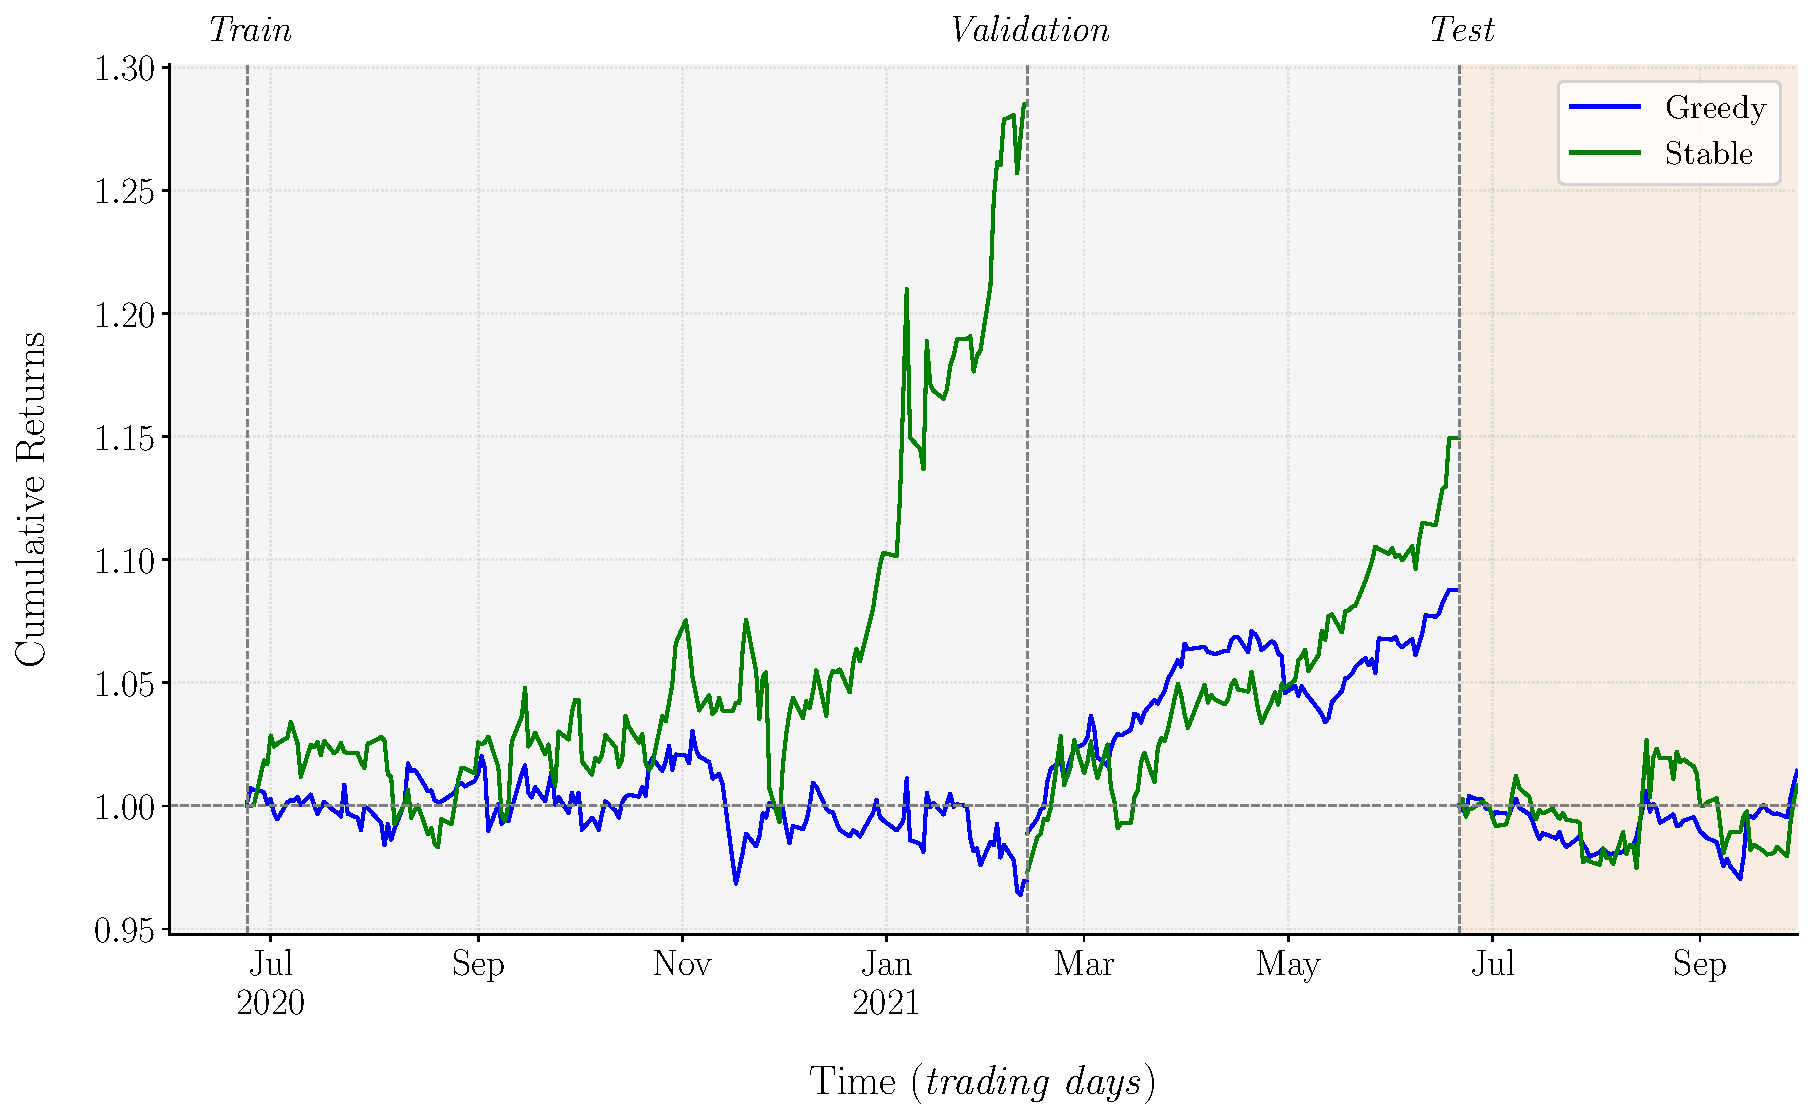
\includegraphics[scale=0.58]{/Users/jesusvillotamiranda/Library/CloudStorage/OneDrive-UniversidaddeLaRioja/CEMFI/__MSc__/__Second_year__/6th_Term/MasterThesis/__Output/KMeans_Portfolio_Cum_Returns_(L=4,theta=0.5k).pdf}
  \subcaption*{\textit{Note: The holding period of the beta-neutral strategies is set to $L$ = 4 trading days and the number of traded clusters is, $\theta = \integer{0.5k}=13$ as we have $k^*=26$ clusters. The selection criteria for these parameters is based on maximizing the Sharpe Ratios of the train and validation samples. The poor out-of-sample performance of the trading strategy indicates that the embeddings-based clusters lack robustness and fail to generalize effectively over time.}}
  \label{fig:KMeans_Portfolio_Cum_Returns}
\end{figure}
%----------------------------------------------------


%\red{The correlation between the trading signals generated by the greedy and stable algorithms is 0.512450. What is the correlation in each data split?
%}


%----------------------------------------------------
\inserthere{tab:KMeans_portfolio_statistics}

\begin{table}[H]
    \caption{Statistics of $\mathcal{P}_{\t{KMeans}}$ across data splits}
    \centering
    \renewcommand{\arraystretch}{0.8}
%    \begin{tabular}{|c|c|c|c|c|c|}
    \begin{tabular}{cccccc}
    	\hline \Xhline{2\arrayrulewidth}
%        \rowcolor{gray!10}
        \textbf{Split} & \textbf{Algorithm} & \textbf{Cum. Return} & \textbf{Avg. Return} & \textbf{St. Deviation} & \textbf{Sharpe Ratio} \\
%        \rowcolor{gray!10}
        & & & \textit{(daily)} & \textit{(daily)} & \textit{(annual)} \\
        \hline \Xhline{2\arrayrulewidth}
        \multirow{2}{*}{All}       & \textit{Greedy} & 1.070 & 0.021 & 0.006 & 0.54 \\        & \textit{Stable} & 1.489 & 0.121 & 0.011 & 1.82 \\         \hline          \multirow{2}{*}{Train}       & \textit{Greedy} & 0.969 & -0.019 & 0.007 & -0.41 \\        & \textit{Stable} & 1.285 & 0.151 & 0.012 & 1.97 \\         \hline          \multirow{2}{*}{Validation}       & \textit{Greedy} & 1.088 & 0.094 & 0.005 & 3.23 \\        & \textit{Stable} & 1.149 & 0.155 & 0.008 & 2.93 \\         \hline          \multirow{2}{*}{Test}       & \textit{Greedy} & 1.014 & 0.019 & 0.004 & 0.70 \\        & \textit{Stable} & 1.008 & 0.011 & 0.009 & 0.20 \\         \hline \Xhline{2\arrayrulewidth}
    \end{tabular}
    \label{tab:KMeans_portfolio_statistics}
\vspace{0.5cm}
\subcaption*{\textit{Note: Portfolio statistics of the trading strategy based on clusters obtained from applying KMeans to article embeddings. The statistics provided are: Cumulative Return, Average Return, Standard Deviation and Sharpe Ratio, which have been computed in accordance to the formulas provided in the text. Such statistics are provided for both cluster-selection algorithms: Greedy and Stable. The Greedy algorithm longs (shorts) clusters that maximize (minimize) the cluster-average-$SR$ in the validation sample subject to a positivity (negativity) constraint, while the Stable algorithm longs (shorts) clusters that minimize the rank difference between the training and validation rankings of the cluster-average-$SR$'s subject to a positivity (negativity) constraint, which is now imposed on both sample splits. In both algorithms, the cardinality of each leg is upper-bounded by a hyperparameter $\theta$. 
The holding period of the beta-neutral positions is set to $L$ = 4 trading days and the number of traded clusters is, $\theta = 0.5k=13$ as there are $k^*=26$ KMeans clusters of article embeddings. The selection criteria for these hyperparameters ($L,\theta$) is based on maximizing the Sharpe Ratios of the train and validation samples.
} }
\end{table}
%----------------------------------------------------

%%%%%%%%%%%%%%%%%%%%%%%%%%%%%%%%%%%%%%%%%%%%%%%%%%%%%
%%%%%%%%%%%%%%%%%%%%%%%%%%%%%%%%%%%%%%%%%%%%%%%%%%%%%
%%%%%%%%%%%%%%%%%%%%%  LLM  %%%%%%%%%%%%%%%%%%%%%%%%%
%%%%%%%%%%%%%%%%%%%%%%%%%%%%%%%%%%%%%%%%%%%%%%%%%%%%%
%%%%%%%%%%%%%%%%%%%%%%%%%%%%%%%%%%%%%%%%%%%%%%%%%%%%%

%\bblue{\noindent \Vhrulefill
%
%\noindent \Vhrulefill [~~LLM~~] \Vhrulefill
%
%\noindent \Vhrulefill}

\mx 
In \cref{fig:LLM_portfolio_returns} we plot the cumulative returns of the portfolio based on LLM clustering ($\mathcal P_{LLM}$). As before, both algorithms perform really well on ``seen'' data. However, different from before, the \textit{Greedy} algorithm works well also on the Training Split (which it was not trained on). More importantly, both algorithms do a great job in the test data. As we can see, both are able to achieve a consistent profile of earnings through the split. 
%In this case, the correlation of the trading signals generated by both algorithms is higher (0.693)
%
%\mx 
The summary statistics of the portfolio are provided in \cref{tab:LLM_portfolio_statistics}, where we see confirmed the fact that both algorithms excel at 
%generating profits out of sample. 
anticipating the market out of sample. 

%----------------------- PLOT ----------------------
\inserthere{fig:LLM_portfolio_returns}
\begin{figure}[H]
  \centering
    \caption{Cumulative Returns of $\mathcal P_{LLM}$ across data splits for LLM-based clustering}
  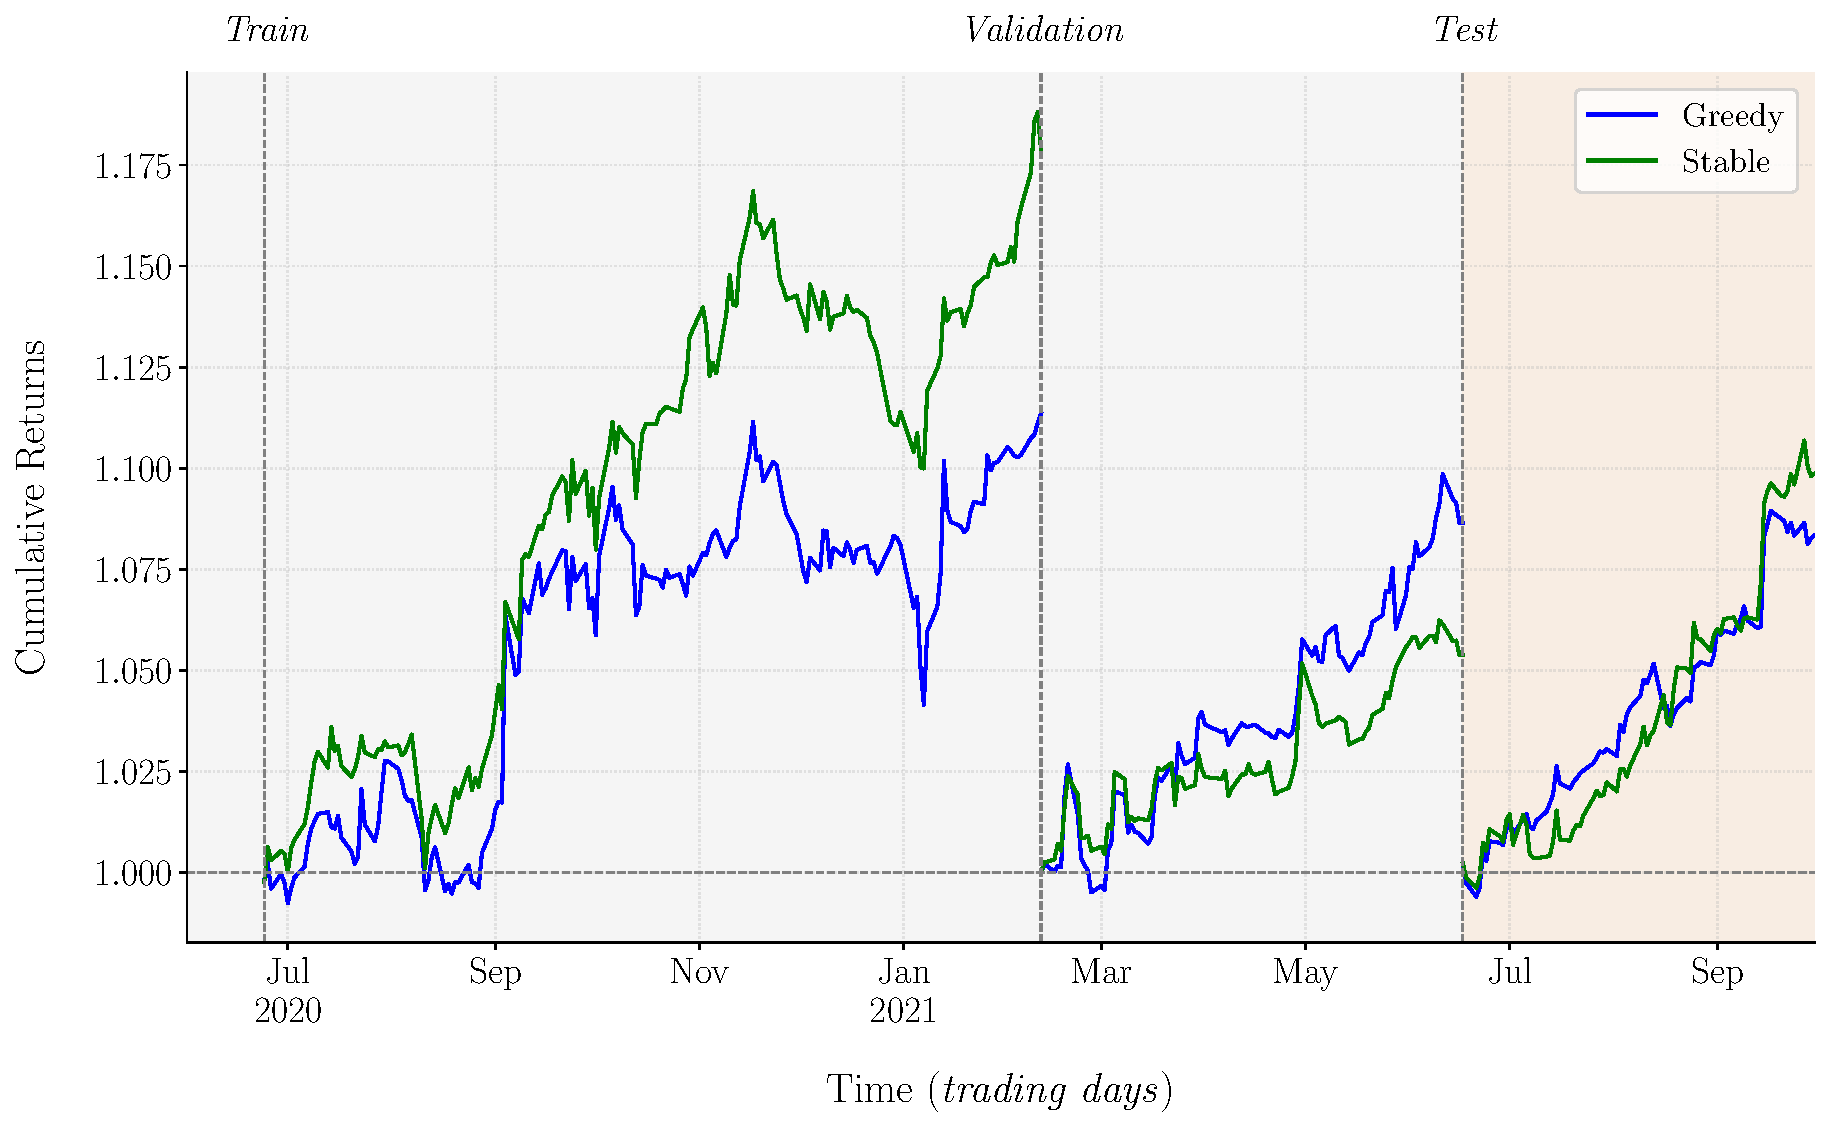
\includegraphics[scale=0.58]{/Users/jesusvillotamiranda/Library/CloudStorage/OneDrive-UniversidaddeLaRioja/CEMFI/__MSc__/__Second_year__/6th_Term/MasterThesis/__Output/LLAMA_Portfolio_Cum_Returns_(L=4,theta=0.5k).pdf}
  \subcaption*{\textit{Note: The holding period of the beta-neutral strategies is set to $L=4$ trading days and the number of traded clusters is  $\theta=\integer{0.5k}=10$, as now we have $k=20$ clusters. The selection criteria for these parameters is based on maximizing the Sharpe Ratios of the train and validation samples. 
%The good performance of the trading strategy out of sample indicates that our proposed LLM-based clusters deliver insights into predicting market reactions to news-implied firm-specific economic shocks.
The strong out-of-sample performance of the trading strategy suggests that our proposed LLM-based clusters effectively provide insights for predicting market reactions to firm-specific economic shocks implied by news.
}}
  \label{fig:LLM_portfolio_returns}
\end{figure}
%----------------------------------------------------


%\blue{
%\begin{itemize}
% \item The cumulative returns of the portfolio obtained by applying our selection algorithms to the LLM clusters is plotted in \cref{fig:LLM_portfolio_returns}. As we can see, different from before, now the portfolio does surprisingly well on unseen data (test set). 
%  \item The visual results of the plot, are confirmed by the statistics of the portfolio, which we can see in \cref{tab:LLM_portfolio_statistics}.
%  \item The correlation betweent he trading signals generated by the greedy and stable algorithm are, in this case, 0.693604
%\end{itemize}
%
%}

%--------------------- TABLE ------------------------
\inserthere{tab:LLM_portfolio_statistics}

\begin{table}[H]
    \caption{Statistics of $\mathcal{P}_{LLM}$ across data splits}
    \centering
    \renewcommand{\arraystretch}{0.8}
    \begin{tabular}{cccccc}
        \hline \Xhline{2\arrayrulewidth}
%        \rowcolor{gray!10}
        \textbf{Split} & \textbf{Algorithm} & \textbf{Cum. Return} & \textbf{Avg. Return} & \textbf{St. Deviation} & \textbf{Sharpe Ratio} \\
%        \rowcolor{gray!10}
        & & & \textit{(daily)} & \textit{(daily)} & \textit{(annual)} \\
		\hline \Xhline{2\arrayrulewidth}
        \multirow{2}{*}{All}       & \textit{Greedy} & 1.311 & 0.082 & 0.006 & 2.17 \\        & \textit{Stable} & 1.365 & 0.095 & 0.005 & 2.78 \\         \hline          \multirow{2}{*}{Train}       & \textit{Greedy} & 1.113 & 0.065 & 0.007 & 1.44 \\        & \textit{Stable} & 1.179 & 0.100 & 0.006 & 2.53 \\         \hline          \multirow{2}{*}{Validation}       & \textit{Greedy} & 1.086 & 0.093 & 0.005 & 2.86 \\        & \textit{Stable} & 1.054 & 0.059 & 0.004 & 2.16 \\         \hline          \multirow{2}{*}{Test}       & \textit{Greedy} & 1.083 & 0.105 & 0.004 & 4.30 \\        & \textit{Stable} & 1.099 & 0.124 & 0.004 & 4.38 \\         \hline \Xhline{2\arrayrulewidth}
    \end{tabular}
    \label{tab:LLM_portfolio_statistics}
\vspace{0.5cm}
\subcaption*{\textit{Note: Portfolio statistics of the trading strategy applied to the LLM clusters. The statistics provided are: Cumulative Return, Average Return, Standard Deviation and Sharpe Ratio, which have been computed in accordance to the formulas provided in the text. Such statistics are provided for both cluster-selection algorithms: Greedy and Stable. The Greedy algorithm longs (shorts) clusters that maximize (minimize) the cluster-average-$SR$ in the validation sample subject to a positivity (negativity) constraint, while the Stable algorithm longs (shorts) clusters that minimize the rank difference between the training and validation rankings of the cluster-average-$SR$'s subject to a positivity (negativity) constraint, which is now imposed on both sample splits. In both algorithms, the cardinality of each leg is upper-bounded by a hyperparameter $\theta$. 
The holding period of the beta-neutral positions is set to $L$ = 4 trading days and the number of traded clusters is, $\theta = 0.5k=13$ as there are $k^*=26$ KMeans clusters of article embeddings. The selection criteria for these hyperparameters ($L,\theta$) is based on maximizing the Sharpe Ratios of the train and validation samples.
}}
\end{table}
%----------------------------------------------------

